%%%%%%%%%%%%%%%%%%%%%%%%%%%%%%%%%%%%%%%
% Programming/Coding Assignment
% LaTeX Template
%
% This template has been downloaded from:
% http://www.latextemplates.com
%
% Original author:
% Ted Pavlic (http://www.tedpavlic.com)
%
% Note:
% The \lipsum[#] commands throughout this template generate dummy text
% to fill the template out. These commands should all be removed when 
% writing assignment content.
%
% This template uses a Perl script as an example snippet of code, most other
% languages are also usable. Configure them in the "CODE INCLUSION 
% CONFIGURATION" section.
%
%%%%%%%%%%%%%%%%%%%%%%%%%%%%%%%%%%%%%%%%%

%----------------------------------------------------------------------------------------
%	PACKAGES AND OTHER DOCUMENT CONFIGURATIONS
%----------------------------------------------------------------------------------------

\documentclass[a4paper]{article}

\usepackage{fancyhdr} % Required for custom headers
\usepackage{lastpage} % Required to determine the last page for the footer
\usepackage{extramarks} % Required for headers and footers
\usepackage[usenames,dvipsnames]{color} % Required for custom colors
\usepackage{graphicx} % Required to insert images
\usepackage{listings} % Required for insertion of code
\renewcommand*{\lstlistingname}{代码} % change "Listing <ref> to 代码 <ref>
\usepackage{courier} % Required for the courier font
\usepackage{lipsum} % Used for inserting dummy 'Lorem ipsum' text into the template

\usepackage[UTF8]{ctex} % Required for Chinese character
\usepackage{tocloft} % Required for beautiful toc
\usepackage[colorlinks]{hyperref} % Required for clickable toc
\hypersetup{
    colorlinks=false,
    citecolor=red,
    filecolor=black,
    linkcolor=blue,
    urlcolor=black,
    linkbordercolor	= {1 0 0}
}
\usepackage[title]{appendix} % Required for appendix
\usepackage{float}
\usepackage{amsmath} % used for \text{} in math formula


% used for beautiful table
\usepackage{booktabs} 
\usepackage[T1]{fontenc}
\usepackage{tabu}
\usepackage{longtable}
\usepackage[table]{xcolor}

\usepackage{algpseudocode}
\usepackage{algorithm}

%used for beautiful order list
\usepackage{enumitem}

\def\equationautorefname{式}%
\def\footnoteautorefname{脚注}%
\def\itemautorefname{项}%
\def\figureautorefname{图}%
\def\tableautorefname{表}%
\def\partautorefname{篇}%
\def\appendixautorefname{附录}%
\def\chapterautorefname{章}%
\def\sectionautorefname{节}%
\def\subsectionautorefname{小节}%
\def\subsubsectionautorefname{subsubsection}%
\def\paragraphautorefname{段落}%
\def\subparagraphautorefname{子段落}%
\def\FancyVerbLineautorefname{行}%
\def\theoremautorefname{定理}%
\def\algorithmautorefname{算法}
\let\subsubsectionautorefname\sectionautorefname

% TODO:
\newcommand{\aref}[1]{\hyperref[#1]{附录~\ref{#1}}}

% Margins
\topmargin=-0.45in
\evensidemargin=0in
\oddsidemargin=0in
\textwidth=6.5in
\textheight=9.0in
\headsep=0.25in

\linespread{1.1} % Line spacing

% Set up the header and footer
\pagestyle{fancy}
\lhead{\hmwkAuthorName} % Top left header
\chead{\hmwkClass\ (\hmwkClassInstructor\ \hmwkClassTime): \hmwkTitle} % Top center head
\rhead{\firstxmark} % Top right header
\lfoot{\lastxmark} % Bottom left footer
\cfoot{} % Bottom center footer
\rfoot{Page\ \thepage\ of\ \protect\pageref*{LastPage}} % Bottom right footer
\renewcommand\headrulewidth{0.4pt} % Size of the header rule
\renewcommand\footrulewidth{0.4pt} % Size of the footer rule

\setlength\parindent{0pt} % Removes all indentation from paragraphs

%----------------------------------------------------------------------------------------
%	CODE INCLUSION CONFIGURATION
%----------------------------------------------------------------------------------------

\definecolor{MyDarkGreen}{rgb}{0.0,0.4,0.0} % This is the color used for comments
% \lstloadlanguages{c} % Load Perl syntax for listings, for a list of other languages supported see: ftp://ftp.tex.ac.uk/tex-archive/macros/latex/contrib/listings/listings.pdf
% \lstset{language=sql, % Use Perl in this example
%         frame=single, % Single frame around code
%         basicstyle=\small\ttfamily, % Use small true type font
%         keywordstyle=[1]\color{Blue}, % Perl functions bold and blue
%         keywordstyle=[2]\color{Purple}, % Perl function arguments purple
%         keywordstyle=[3]\color{Blue}\underbar, % Custom functions underlined and blue
%         identifierstyle=, % Nothing special about identifiers                                         
%         commentstyle=\usefont{T1}{pcr}{m}{sl}\color{MyDarkGreen}\small, % Comments small dark green courier font
%         stringstyle=\color{Purple}, % Strings are purple
%         showstringspaces=false, % Don't put marks in string spaces
%         tabsize=4, % 5 spaces per tab
%         %
%         % Put standard Perl functions not included in the default language here
%         % morekeywords={rand},
%         morekeywords={rand, go},
%         %
%         % Put Perl function parameters here
%         morekeywords=[2]{REAL},
%         %
%         % Put user defined functions here
%         morekeywords=[3]{},
%        	%
%         morecomment=[l][\color{Blue}]{...}, % Line continuation (...) like blue comment
%         numbers=left, % Line numbers on left
%         firstnumber=1, % Line numbers start with line 1
%         numberstyle=\tiny\color{Blue}, % Line numbers are blue and small
%         stepnumber=2, % Line numbers go in steps of 5,
%         firstnumber=1
% }

\lstloadlanguages{Python}
\lstdefinestyle{mypython}{
    language=Python, % Use Perl in this example
    frame=single, % Single frame around code
    basicstyle=\small\ttfamily, % Use small true type font
    keywordstyle=[1]\color{Blue}, % Perl functions bold and blue
    keywordstyle=[2]\color{Purple}, % Perl function arguments purple
    keywordstyle=[3]\color{Blue}\underbar, % Custom functions underlined and blue
    keywordstyle=[4]\color{Aquamarine}, % Custom functions underlined and blue
    identifierstyle=, % Nothing special about identifiers                                         
    commentstyle=\usefont{T1}{pcr}{m}{sl}\color{MyDarkGreen}\small, % Comments small dark green courier font
    stringstyle=\color{Purple}, % Strings are purple
    showstringspaces=false, % Don't put marks in string spaces
    tabsize=4, % 5 spaces per tab
    %
    % Put standard Perl functions not included in the default language here
    % morekeywords={rand},
    morekeywords={go, REFERENCES, DATABASE, SCHEMA},
    %
    % Put Perl function parameters here
    morekeywords=[4]{np},
    %
    % Put user defined functions here
    morekeywords=[1]{self},
    morekeywords=[3]{},
    %
    morecomment=[l][\color{Blue}]{...}, % Line continuation (...) like blue comment
    numbers=left, % Line numbers on left
    firstnumber=1, % Line numbers start with line 1
    numberstyle=\tiny\color{Blue}, % Line numbers are blue and small
    stepnumber=2, % Line numbers go in steps of 5,
    firstnumber=1
}
% Creates a new command to include a perl script, the first parameter is the filename of the script (without .pl), the second parameter is the caption
\lstloadlanguages{bash}
\lstdefinestyle{mybash}{
    language=bash, % Use Perl in this example
    frame=single, % Single frame around code
    basicstyle=\small\ttfamily, % Use small true type font
    keywordstyle=[1]\color{Blue}, % Perl functions bold and blue
    keywordstyle=[2]\color{Purple}, % Perl function arguments purple
    keywordstyle=[3]\color{Blue}\underbar, % Custom functions underlined and blue
    keywordstyle=[4]\color{Aquamarine}, % Custom functions underlined and blue
    identifierstyle=, % Nothing special about identifiers                                         
    commentstyle=\usefont{T1}{pcr}{m}{sl}\color{MyDarkGreen}\small, % Comments small dark green courier font
    stringstyle=\color{Purple}, % Strings are purple
    showstringspaces=false, % Don't put marks in string spaces
    tabsize=4, % 5 spaces per tab
    %
    % Put standard Perl functions not included in the default language here
    % morekeywords={rand},
    morekeywords={go, REFERENCES, DATABASE, SCHEMA},
    %
    % Put Perl function parameters here
    morekeywords=[4]{np},
    %
    % Put user defined functions here
    morekeywords=[1]{self, conda, sudo, python, bash},
    morekeywords=[3]{},
    %
    morecomment=[l][\color{Blue}]{...}, % Line continuation (...) like blue comment
    numbers=left, % Line numbers on left
    firstnumber=1, % Line numbers start with line 1
    numberstyle=\tiny\color{Blue}, % Line numbers are blue and small
    stepnumber=2, % Line numbers go in steps of 5,
    firstnumber=1
}

\newcommand{\shfilescript}[3]{
\begin{itemize}
\item[]\lstinputlisting[caption=#2, label=lst:#1, language=sh]{#3}
\end{itemize}
}
\newcommand{\shscript}[3]{
\begin{itemize}
\item[]\begin{lstlisting}[label=lst:#1, caption=#2] #3 \end{lstlisting}
\end{itemize}
}

%----------------------------------------------------------------------------------------
%	DOCUMENT STRUCTURE COMMANDS
%	Skip this unless you know what you're doing
%----------------------------------------------------------------------------------------

% Header and footer for when a page split occurs within a problem environment
\newcommand{\enterProblemHeader}[1]{
\nobreak\extramarks{#1}{#1 见下页\ldots}\nobreak{} 
\nobreak\extramarks{接上页}{#1 见下页\ldots}\nobreak{}
}

% Header and footer for when a page split occurs between problem environments
\newcommand{\exitProblemHeader}[1]{
\nobreak\extramarks{接上页}{#1 见下页\ldots}\nobreak{}
\nobreak\extramarks{#1}{}\nobreak{}
}
% TODO:code here enable the number before section, but it disable the numbering of problems
%\setcounter{secnumdepth}{0} % Removes default section numbers
\newcounter{homeworkProblemCounter} % Creates a counter to keep track of the number of problems

\newcommand{\homeworkProblemName}{}
\newenvironment{homeworkProblem}[1][Problem \arabic{homeworkProblemCounter}]{ % Makes a new environment called homeworkProblem which takes 1 argument (custom name) but the default is "Problem #"
\stepcounter{homeworkProblemCounter} % Increase counter for number of problems
\renewcommand{\homeworkProblemName}{#1} % Assign \homeworkProblemName the name of the problem
\section{\homeworkProblemName} % Make a section in the document with the custom problem count
\enterProblemHeader{\homeworkProblemName} % Header and footer within the environment
}{
\exitProblemHeader{\homeworkProblemName} % Header and footer after the environment
}

\newcommand{\problemAnswer}[1]{ % Defines the problem answer command with the content as the only argument
\noindent\framebox[\columnwidth][c]{\begin{minipage}{0.98\columnwidth}#1\end{minipage}} % Makes the box around the problem answer and puts the content inside
}

\newcommand{\homeworkSectionName}{}
\newenvironment{homeworkSection}[1]{ % New environment for sections within homework problems, takes 1 argument - the name of the section
\renewcommand{\homeworkSectionName}{#1} % Assign \homeworkSectionName to the name of the section from the environment argument
\subsection{\homeworkSectionName} % Make a subsection with the custom name of the subsection
\enterProblemHeader{\homeworkProblemName\ [\homeworkSectionName]} % Header and footer within the environment
}{
\enterProblemHeader{\homeworkProblemName} % Header and footer after the environment
}


\newcommand{\codev}[1]{\textsf{#1}}
%----------------------------------------------------------------------------------------
%	NAME AND CLASS SECTION
%----------------------------------------------------------------------------------------

% table color
\definecolor{tableHeader}{RGB}{245, 245, 245}
\definecolor{tableLineOne}{RGB}{245, 245, 245}
\definecolor{tableLineTwo}{RGB}{224, 224, 224}
\newcommand{\tableHeaderStyle}{
    \rowfont{\leavevmode\color{white}\bfseries}
    \rowcolor{tableHeader}
}

%----------------------------------------------------------------------------------------

\newcommand{\hmwkTitle}{project-name\ \#2} % Assignment title
\newcommand{\hmwkDueDate}{Tuesday,\ September\ 18,\ 2018} % Due date
\newcommand{\hmwkClass}{16级计科\ 7班} % Course/class
\newcommand{\hmwkClassTime}{周三3-4节} % Class/lecture time
\newcommand{\hmwkClassInstructor}{teacher-name} % Teacher/lecturer
\newcommand{\hmwkAuthorName}{颜彬} % Your name
\newcommand{\hmwkAuthorId}{16337269} % Your id 

%----------------------------------------------------------------------------------------
%	TITLE PAGE
%----------------------------------------------------------------------------------------

\usepackage{titling}

\title{
\vspace{2in}
\textmd{\textbf{\hmwkClass:\ \hmwkTitle}}\\
\normalsize\vspace{0.1in}\small{Due\ on\ \hmwkDueDate}\\
\vspace{0.1in}\large{\textit{\hmwkClassInstructor\ \hmwkClassTime}}
\vspace{3in}
}

\author{\textbf{\LARGE{\hmwkAuthorName}} \\ \\ \textbf{\LARGE{\hmwkAuthorId}}}
\date{} % Insert date here if you want it to appear below your name
%----------------------------------------------------------------------------------------

\begin{document}
% \begin{titlingpage} % This is for ignore page number in first page. package titling

\maketitle

%----------------------------------------------------------------------------------------
%	TABLE OF CONTENTS
%----------------------------------------------------------------------------------------

% \setcounter{tocdepth}{2} % Uncomment this line if you don't want subsections listed in the ToC
% set depth in toc

% \renewcommand{\cftsecleader}{\cftdotfill{\cftdotsep}} % used for dots between <section> and <page>

\renewcommand{\contentsname}{Content} % force the word to be "content
\newpage
\tableofcontents
\addtocontents{toc}{~\hfill\textbf{Page}\par}
\newpage

% below are document body


% To have just one problem per page, simply put a \clearpage after each problem
\section{项目简介}
这次项目实现了名为SDFS(Simple Distributed File System)的分布式文件系统工具。\\

其代码包括server端和client端。在client端,
用户可以执行文件系统支持的常用操作,例如上传文件(到SDFS)、下载文件(回原来的fs)、ls、cat等。server端负责响应
这些请求并做相关的操作。(\autoref{fig:intro}为其命令行界面,展示了支持的一些操作)。\\

本项目使用Python 3.7实现,仅仅利用了Python的标准库和rpyc库,其中后者用于发起rpc请求。整个分布式文件系统
以rpc的方式交互和传递信息。\\

\begin{figure}[!hbt]
    \begin{center}
    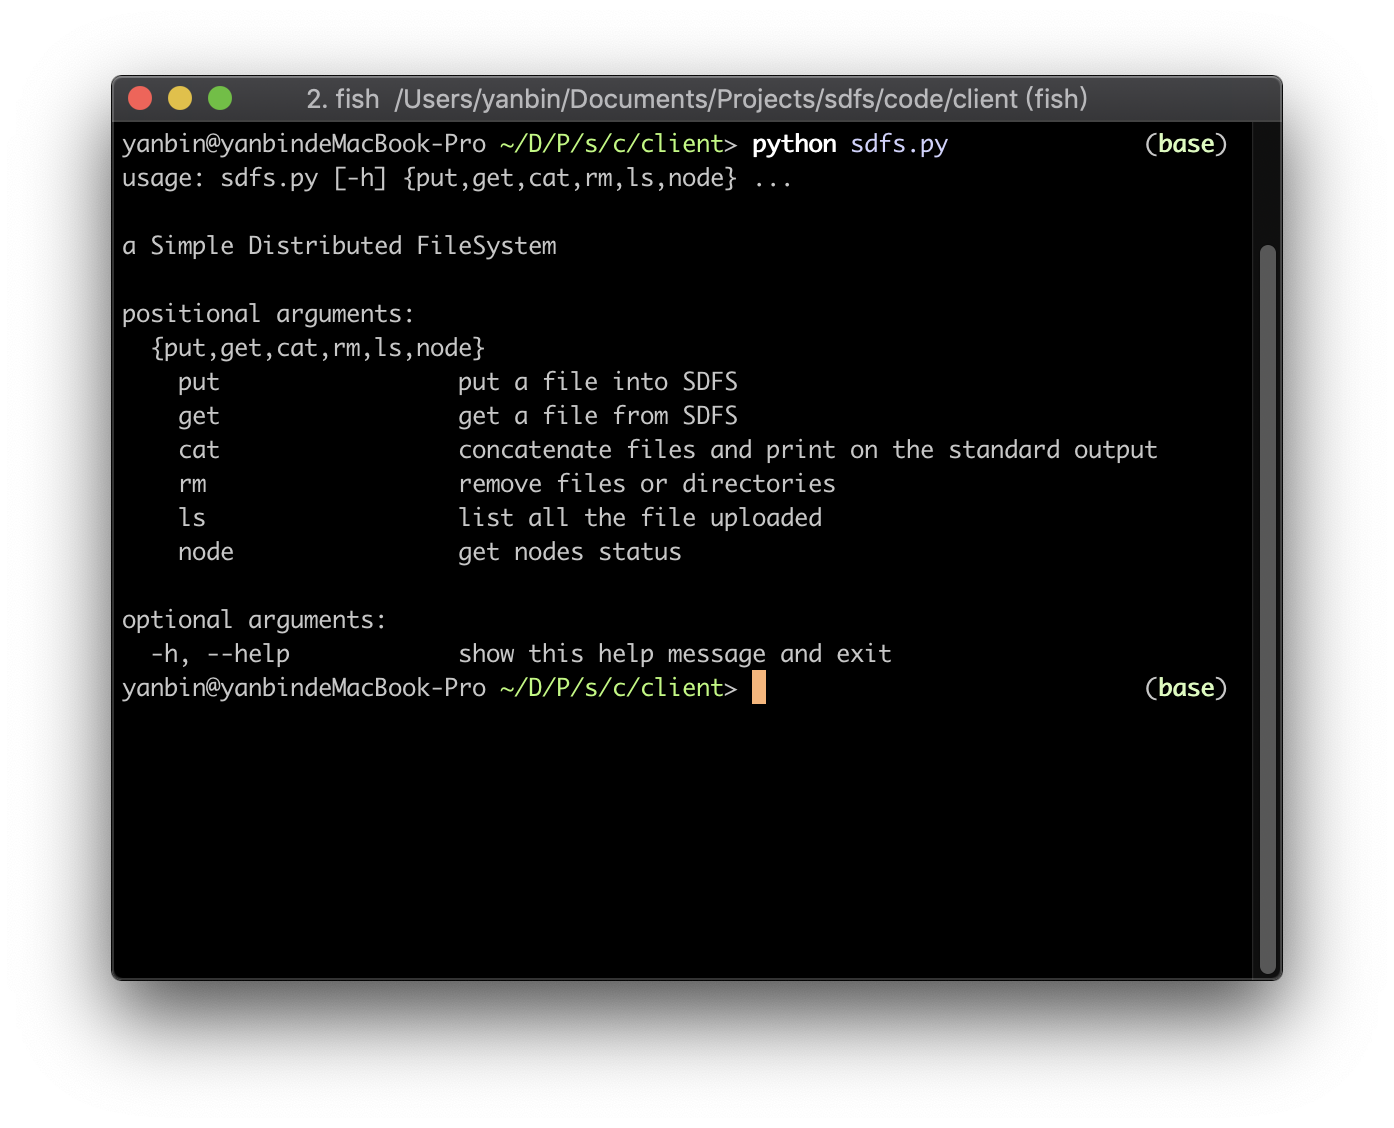
\includegraphics[scale=0.5]{assets/intro.png}
    \caption{SDFS命令行界面\label{fig:intro}} 
    \end{center} 
\end{figure} 

\section{使用方式}
\subsection{开发环境介绍}
使用Python 3.7开发,使用了rpyc第三方库。如果系统有预装conda,可以按\autoref{lst:install}的方式配置。
测试环境下,会同时开启多个终端并运行多个进程,需要使用tmux工具。\\

其他安装方式与之类似。\\

\begin{figure}[!hbt]
\begin{itemize}
\item[] \begin{lstlisting}[style=mybash, label=lst:install, caption=环境安装方式]
sudo apt install tmux
conda create --name sdfs python=3.7
conda install rpyc
conda activate sdfs
\end{lstlisting}
\end{itemize}
\end{figure}
\subsection{服务端运行方式}
服务端需要运行起注册服务器、NameNode和DataNode(见\autoref{sec:arch}的介绍)。如\autoref{lst:run}所示。\\

其中run.sh程序需要安装tmux工具。
\begin{figure}[!hbt]
\begin{itemize}
\item[] \begin{lstlisting}[style=mybash, label=lst:run, caption=测试环境下服务端的运行方式]
cd code/server
python rpyc_registry.py # 运行注册服务
bash run.sh # 运行NameNode和DataNode
\end{lstlisting}
\end{itemize}
\end{figure}

\subsection{客户端运行方式}
客户端的运行方式如\autoref{lst:client}所示。如果环境正确,预计会看到\autoref{fig:intro}所示的欢迎
画面。该画面展示了命令行工具支持的指令,以及他们的简要用法。
\begin{figure}[!hbt]
\begin{itemize}
\item[] \begin{lstlisting}[style=mybash, label=lst:client, caption=客户端运行方式]
cd code/client
python sdfs.py
\end{lstlisting}
\end{itemize}
\end{figure}

\section{设计架构}\label{sec:arch}
由于本项目尽可能地按照HDFS架构来设计,故先介绍HDFS架构,再比较和本项目的不同之处。
\subsection{HDFS设计架构}
本项目的设计类似于HDFS架构。\autoref{fig:hdfs}介绍了HDFS的
具体架构。\\

在HDFS是一个master/slave架构的文件系统。一个HDFS集群包括一个NameNode和若干个DataNode。其中NameNode是
主服务器,负责管理文件的元数据,例如文件系统的命名空间、文件的访问权限等。其他的若干个DataNode负责存储和管理文件的真实
数据。\\

在HDFS内部,一个文件会划分为多个块(block)。这些不同的块会产生若干个(一般是3个)副本(replica)。这些副本
被分配到不同的DataNode中存储。当用户需要检索某个文件时,需要向不同的DataNode拿到文件的块,再将块拼接
起来得到原始文件。\\

在这个过程中,NameNode会负责处理打开文件、关闭文件、文件重命名以及处理文件的路径。除此之外,NameNode还负责
将副本(replica of blocks)映射到某个DataNode中。\\

DataNode的任务简化为创建块、删除块、以及根据NameNode的指示复制块等。

\begin{figure}[!hbt]
    \begin{center}
    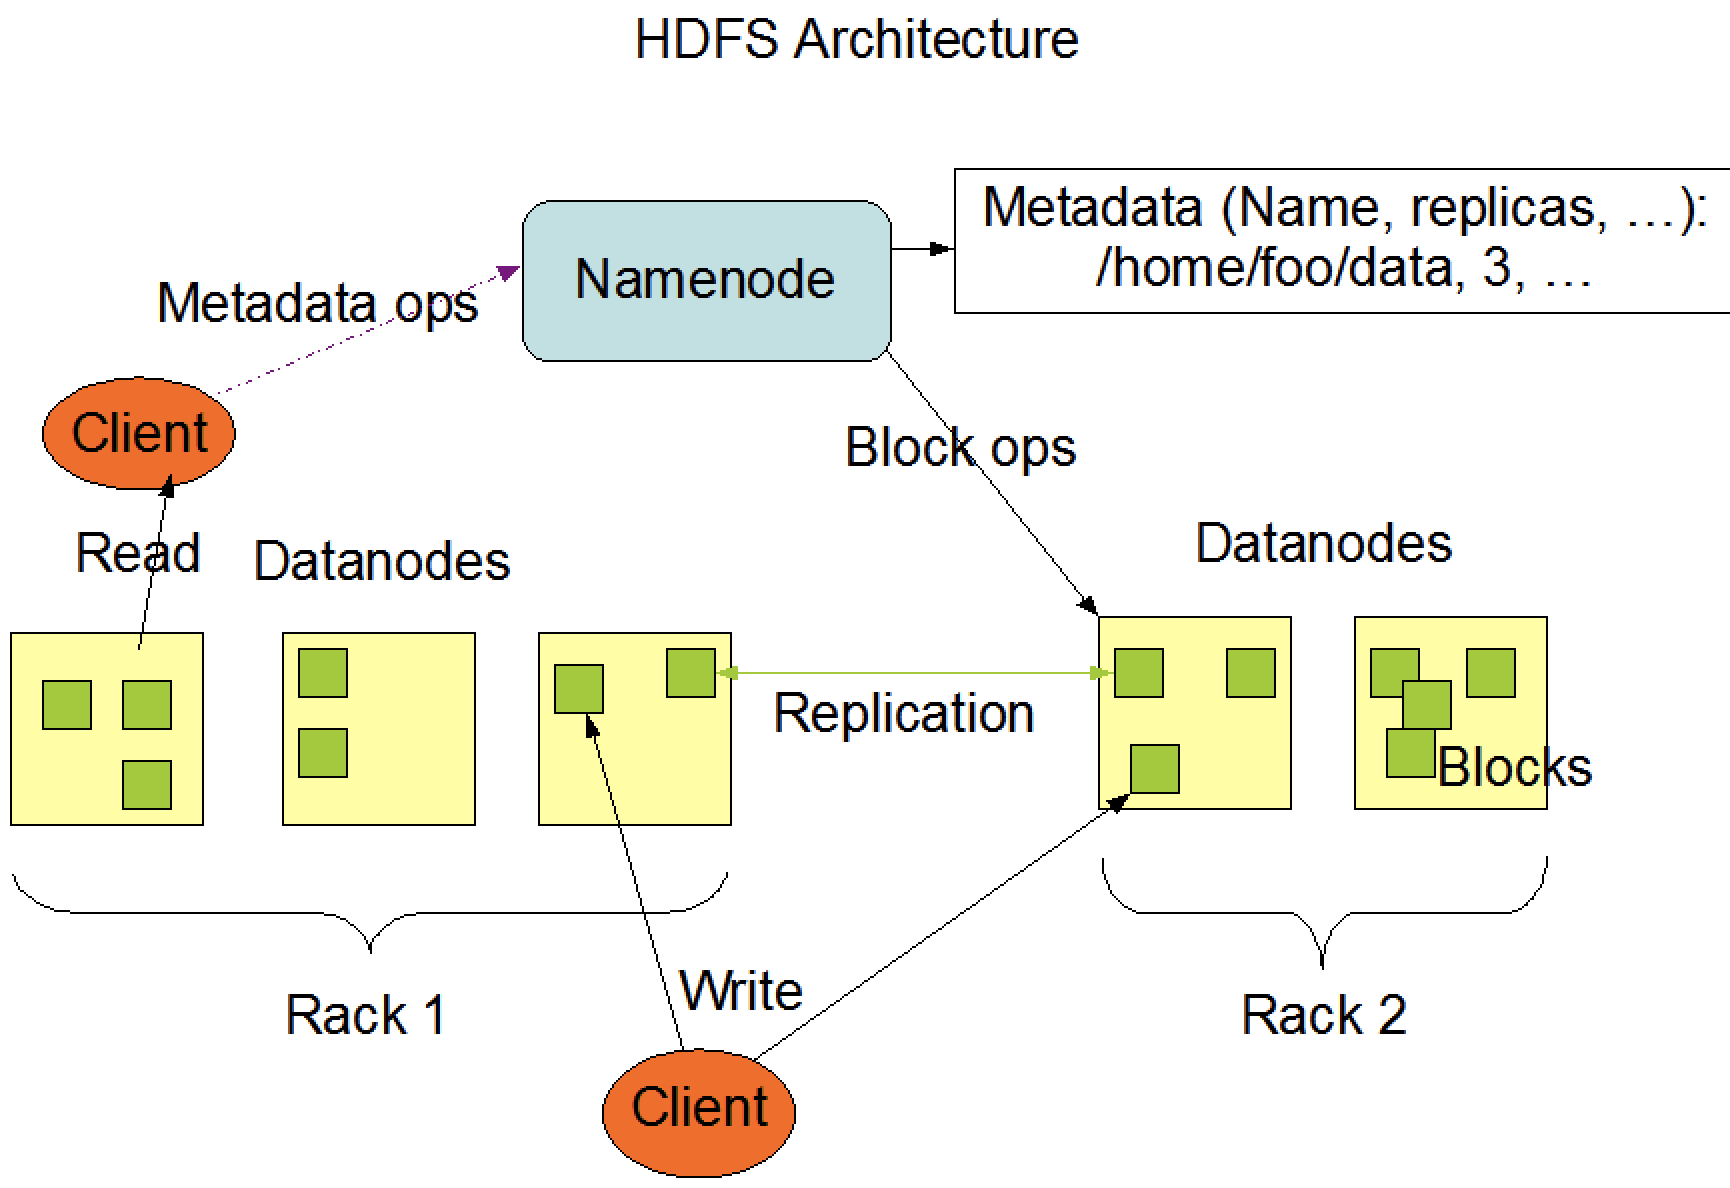
\includegraphics[scale=0.3]{assets/hdfs.png}
    \caption{HDFS架构示意图\label{fig:hdfs}} 
    \end{center} 
\end{figure} 
\subsection{SDFS设计架构}
本项目(SDFS)的架构与HDFS十分类似,但HDFS还是过于复杂,作为一次课程项目,做了如下的简化。
\begin{itemize}
    \item 不存储文件路径。即SDFS是``扁平化''的文件系统,所有文件存储在根目录上。
    \item 不进行用户权限管理。即默认所有用户是root用户,具有完全的权限。
\end{itemize}
但SDFS支持并实现了HDFS的许多功能,包括文件分块、为块创建副本、容错、块状态维护和错误块修复等。这些特性保证了
SDFS具有比较好的容错能力。\\

在默认3副本的情况下,任何块可以拥有1-容错的能力。即便一个文件的每个块都有一个副本被损坏了,剩下的两个副本可以
通过投票胜出,成为正确(healthy)的块,从而被用户访问到。\\

假设不考虑块损坏,由于块拥有3个副本,(最坏下)任何两台服务器的停止失效都不会影响到块的正常访问。\\

SDFS还提供了足够的命令行指令,允许用户指定块大小(--block, -b)和指定副本个数(--replica)等。

\subsection{SDFS架构细节}
下面进一步介绍SDFS架构的细节。\\

用户(client)通过命令行工具与HDFS后端交互。后端包括一个注册器(register), 一个NameNode主服务器和若干个
DataNode数据存储器。\\

\subsubsection{启动SDFS}
注册器必须是最开始运行的进程。在注册器启动完毕后,其他后端服务器才可以创建和运行。这些服务进程创建时,
会自动通过广播的方式向注册器进行注册。注册器维护当前活跃的服务进程。\\

由于注册器的存在,NameNode、DataNode和Client三者的交互可以通过注册器完成。任何一方要访问另一方时,
只需要通过rpc向注册器询问一个\emph{服务},注册器会返回该服务的一系列地址(ip和端口)。在这里,NameNode、
DataNode、Client都是服务,它们的``服务标志符''就是自己的名字。\\

如果NameNode、DataNode或Client中有部分进程不在一个子网中,注册器会失效。此时SDFS提供了配置文件的机制,可以
通过配置文件指定要访问的服务的ip和port。
\subsection{发起请求}
当Client实际上由两部分组成。分别是
\begin{itemize}
    \item Parser,命令行解析工具,将用户的输入提取为一个object。
    \item Connector,连接工具,负责使用与NameNode或DataNode作连接和数据传输。
\end{itemize}
当Client发起请求时,Connector拿到解析好的用户输入指令后,要考虑与哪些服务建立连接。\\

其中Client的每个操作都一定要与NameNode建立连接。这是因为所有的``文件分块信息''都被存储到NameNode上,
对文件的任何操作在访问到文件的块之前,都必须向NameNode询问块的所在位置。\\

Client的每个操作都会涉及到一定数量的DataNode。这取决于文件块所在的位置。\\

\emph{Note: Client直接将文件块传送给DataNode,而不是先把文件传给NameNode再由其进行分发。这样做的目的
是尽可能地减少带宽(与HDFS的实现相同)。} \\

具体地说,当执行文件上传(put)操作时,首先Client会向NameNode发起请求,NameNode会告知Client应该把文件的
每个块分配到哪些DataNode上。Client拿到这个信息后,会依次联系DataNode并向其传送对应的块。每传送成功一个DataNode,
Client就要向NameNode告知一次成功,NameNode记录下这个副本的所在位置。\\

如果中途出现了异常,Client会停止操作,并向用户返回错误信息。
但之前传送成功的块不会被丢失。\\

在最坏情况下,Client向DataNode传送了
块后就出现异常,不能成功地向NameNode注册。这种情况的最坏后果也只是同一个块多次地上传到同一个DataNode中,
不会带来数据丢失等恶性后果。这个设计遵循了``至少一次''。

\subsection{信息存储}
显然NameNode和DataNode需要具有存储能力。SDFS的实现是让NameNode和DataNode将信息存储到本地
文件系统的文件中。\\

当DataNode收到某个块后,它会产生一个特殊命名的存储文件。这个存储文件的命名由(原文件名,块号)唯一决定。 \\

当NameNode收到信息,它会将状态存储到一个对象中,并写入文件以持久化存储。\\

信息存储有一个隐含的``写写冲突''问题。这是因为每个服务事实上是多线程的。在每个rpc请求到来时,rpc库会为此
产生一个线程用以响应。而许多数据是不线程安全的。

\section{模块间的介绍和联系}
\subsection{模块介绍}
本项目用到了以下的模块
\begin{itemize}
    \item parser(code/client/parser.py)。该模块解析命令行输入。
    \item runner(code/client/sdfs.py)。用户的命令行工具。用户直接执行的脚本。
    \item connector(code/client/connector.py)。连接用具。负责和DataNode和NameNode作连接。是
    客户端对复杂逻辑的一层抽象
    \item register(code/server/rpyc\_registry.py)。rpyc库自带的模块,用于服务注册。
    \item NameNode(code/server/namenode.py)。NameNod的核心实现。
    \item DataNode(code/server/datanode.py)。Datanode的核心实现
\end{itemize}
\subsection{模块间的联系}
用户直接调用sdfs.py文件。该文件使用parser作命令行解析,然后调用connector执行实际的任务。connector为sdfs.py 
提供了及其简单的抽象。\\

connector有比较复杂的逻辑。对于不同的操作(例如ls、cat、put等),每个操作构成一个成员函数。它负责实际地
与NameNode和DataNode作数据传送,并进行错误处理,尽可能维持足够高的鲁棒性。\\

NameNode和DataNode在一般情况下不会直接交互(除了NameNode发起的block状态检查)。一般情况下,connector
向NameNode询问到足够的信息后,直接向DataNode请求执行相关的操作。
\section{rpyc库简介}
之所以需要简介rpyc库,是因为其涉及到多线程和服务注册的概念,还一致性的讨论有关。\autoref{lst:rpyc}是rpyc库的一个使用
模板,介绍了它的大致用法。\\

rpyc库要求将任务以类的方式实现。每个类会成为一个服务(service)。\\

rpyc库要求每个类以Service这个单词作为结尾。Service前的部分即为该服务的服务名。每个服务可以实现on\_connect
和on\_disconnect函数。在本项目中,NameNode会在on\_connect中向需要的DataNode作连接,并在on\_disconnect中
对它们作连接的释放。\\

每个成员函数名如果以exposed\_开头,则该函数成为服务提供的api。其他服务可以远程调用该函数(不需要exposed\_部分)。
例如\autoref{lst:rpyc}中暴露了put这个api。\\

产生该服务器使用的是ThreadServer这个函数。它会为每个尝试建立起的rpc请求产生一个新的线程。这意味着
可能会产生写冲突问题。
\begin{figure}[!hbt]
\begin{itemize}
\item[] \begin{lstlisting}[style=mypython, label=lst:rpyc, caption=rpyc库简介]
class NameNodeService(rpyc.Service):
    def __init__(self, storage_path=None):
        # ...

    def on_connect(self, conn):
        print('OPEN - {}'.format(conn))
        # ...
    def on_disconnect(self, conn):
        print('COLSE - {}'.format(conn))
        for conn in self.conns:
            conn.close()
    def exposed_put(self, filename, filesize, replica=3, blocksize=1024):
        '''
        NameNode回应存放文件的方式
        @param filename :: Str 文件名
        ...
        @ret Int, [[Tuple(Str, Int)]], 
        ...
        '''
        # ...
        # return ...

if __name__ == '__main__':
    from rpyc.utils.server import ThreadedServer
    t = ThreadedServer(NameNodeService, port=PORT, protocol_config={
        'allow_public_attrs': True,
    }, auto_register=True)
    print('start at port {}'.format(PORT))
    t.start()
\end{lstlisting}
\end{itemize}
\end{figure}

\section{具体代码}
由于代码比较复杂,此处仅以一个具体操作作为例子,讲述从客户端到底层的代码实现。
\subsection{put操作的分发}
在执行到put操作时,首先sdfs会调用parser解析用户命令,并在connector处作分发(\autoref{lst:put-frontent})。\\

分发实际做的操作是调用connector的put成员函数,并向该函数提供文件名。该文件名指向本地文件系统中的一个实际存在的文件。
对parser的具体调用过程略。
\begin{figure}[!hbt]
\begin{itemize}
\item[] \begin{lstlisting}[style=mypython, label=lst:put-frontend, caption=put命令的解析和分发]
# in code/client/sdfs.py
class Dispatcher:
    def __init__(self):
        # ...
    def parse(self):
        self.args = parser.parse_args()
        self.dispatch()
    def dispatch(self):
        try:
            if self.args.which == 'put':
                success, msg = self.conn.put(self.args.file)
                if not success:
                    self.parser.print_help()
                print(msg)
        # ...
\end{lstlisting}
\end{itemize}
\end{figure}
% TODO:记得把--replica加上

\subsection{connector的执行}
connector的代码(\autoref{lst:connector})展示中省去了函数头注释,原始代码见code/client/connector.py。\\

首先put函数会尝试打开文件filename,并以二进制的形式读入数据。然后connector会尝试远程调用NameNode的put方法。
该方法不会真正执行put,而是会返回这个文件的每个分块应该存储到的DataNode的地址。\\

datanodes可以看做列表的列表。datanodes的第i个元素是一个列表,表示文件的第i块应该放在哪些DataNode中。
在代码的外层for中,遍历datanodes,变量idx指当前执行到文件的第idx块。\\

wrtie\_binary变量存储的是第idx块的具体信息。值得注意的是,文件的最后一块的大小很可能跟前面的n-1块不一样,要特殊处理。\\

对每个块,以及这个块应该存储进的每个DataNode,connector会尝试调用put\_block函数,并向NameNode注册这一put\_block操作。
如果全部操作都正常完成了,则程序错误码0和提示信息。否则返回非0的错误码。

\begin{figure}[!hbt]
\begin{itemize}
\item[] \begin{lstlisting}[style=mypython, label=lst:connector, caption=connector的具体代码]
def put(self, filename, blk_sz=16384, replica=3):
    with open(filename, 'rb') as f:
        binary = f.read()
        size = len(binary)
        namenode_conn = rpyc.connect(self.ip, self.port)
        errno, datanodes = namenode_conn.root.put(filename, 
            size, 
            blocksize=blk_sz, 
            replica=replica)
        if errno == 1:
            return False, 'Not enough DataNode for replica'

        # 告知namenode,并对datanode作IO
        for idx, segment in enumerate(datanodes):
            if (idx + 1) * blk_sz <= size:
                write_binary = binary[idx * blk_sz: (idx + 1) * blk_sz]
            else:
                write_binary = binary[idx * blk_sz :]
            for datanode in segment:
                ip, port = datanode
                conn = rpyc.connect(ip, port)
                # 将该块传给datanode
                errno, msg = conn.root.put_block(filename, idx, write_binary)
                if errno == 1:
                    print('Warning: {}-{} alread exists {} block {}'.
                        format(ip, port, filename, idx))
                namenode_conn.root.put_block_registry(filename, idx, datanode)
    return True, 'success'
\end{lstlisting}
\end{itemize}
\end{figure}

\section{实验总结}
\section{一致性和容错}
% 讲一下锁的问题
\begin{appendices}
\section{参考文献} \label{sec:reference}
\section{伪代码补充} \label{sec:file}

\end{appendices}
\end{document}
